
%% $Id$

\chapter{Presenting theories}

\section{Generating theory browsing information} \label{sec:info}
\index{theory browsing information|bold}

Isabelle is able to generate theory browsing information, including HTML
documents that show a theory's definition, the theorems proved in its ML file
and the relationship with its ancestors and descendants.  Besides the HTML
file that is generated for every theory, Isabelle stores links to all theories
in an index file. These indexes are linked with other indexes to represent the
hierarchic structure of Isabelle's logics.

Isabelle also generates graph files that represent the theory hierarchy of a
logic.  There is a graph browser Java applet embedded in the generated HTML
pages, and also a stand-alone application that allows browsing theory graphs
without having to start a WWW browser first.  The latter version also includes
features such as generating {\sc PostScript} files, which are not available in
the applet version.  See \S\ref{sec:browse} for further information.

\medskip

To generate theory browsing information for logics that are part of the
Isabelle distribution, simply append ``\texttt{-i true}'' to the
\settdx{ISABELLE_USEDIR_OPTIONS} setting before making a logic.  For example,
in order to do this for {\FOL}, first add something like this to your Isabelle
settings file
\begin{ttbox}
ISABELLE_USEDIR_OPTIONS="-i true"
\end{ttbox}
and then change into the \texttt{src/FOL} directory of the Isabelle
distribution and run \texttt{isatool make}, or even \texttt{isatool make all}.

\medskip

The theory browsing information is stored within the directory determined by
the \settdx{ISABELLE_BROWSER_INFO} setting.  The \texttt{index.html} file
located there provides an entry point to all standard Isabelle logics.  A
complete HTML version of all object-logics and examples of the Isabelle
distribution is available at
\begin{center}\small
  \begin{tabular}{l}
    \url{http://www.cl.cam.ac.uk/Research/HVG/Isabelle/library/} \\
    \url{http://isabelle.in.tum.de/library/} \\
  \end{tabular}
\end{center}

\medskip

The generated HTML document of any theory includes all theorems proved in the
corresponding {\ML} file, provided these have been stored properly via
\ttindex{qed}, \ttindex{qed_goal}, \ttindex{qed_goalw}, \ttindex{bind_thm}, or
\ttindex{store_thm}.  Section headings may be included in the presentation via
the {\ML} function
\begin{ttbox}\index{*section}
section: string -> unit
\end{ttbox}

\medskip

In order to present your own theories on the web, simply copy the whole
\texttt{ISABELLE_BROWSER_INFO} directory to your WWW server, after generating
browser info like this:
\begin{ttbox}
isatool usedir -i true HOL Foobar
\end{ttbox}
This assumes that directory \texttt{Foobar} contains some \texttt{ROOT.ML}
file to load all your theories, and {\HOL} is your parent logic image.
Ideally, theory browser information would have been generated for {\HOL}
already.

Alternatively, one may specify an external link to an existing body of HTML
data by giving \texttt{usedir} a \texttt{-P} option like this:
\begin{ttbox}
isatool usedir -i true -P http://isabelle.in.tum.de/library/ HOL Foobar
\end{ttbox}


\section{Browsing theory graphs} \label{sec:browse}
\index{theory graph browser|bold} 

The graph browser is a tool for visualizing dependency graphs of
Isabelle theories. Certain nodes of the graph (i.e.~theories) can be
grouped together in ``directories'', whose contents may be hidden,
thus enabling the user to filter out irrelevant information.  The
browser is written in Java, it can be used both as a stand-alone
application and as an applet.


\subsection{Invoking the graph browser}

The stand-alone version of the graph browser is wrapped up as an
Isabelle tool called \tooldx{browser}:
\begin{ttbox}
Usage: browser [GRAPHFILE]
\end{ttbox}
When no filename is specified, the browser automatically changes to
the directory \texttt{ISABELLE_BROWSER_INFO/graph/data}.

\medskip The applet version of the browser can be invoked by opening
the {\tt index.html} file in the directory
\texttt{ISABELLE_BROWSER_INFO} from your Web browser and selecting
``version for Java capable browsers''.  There is also a link to the
corresponding theory graph in every logic's {\tt index.html} file.


\subsection{Using the graph browser}

The browser's main window, which is shown in figure
\ref{browserwindow}, consists of two subwindows: In the left
subwindow, the directory tree is displayed. The graph itself is
displayed in the right subwindow.
\begin{figure}[h]
  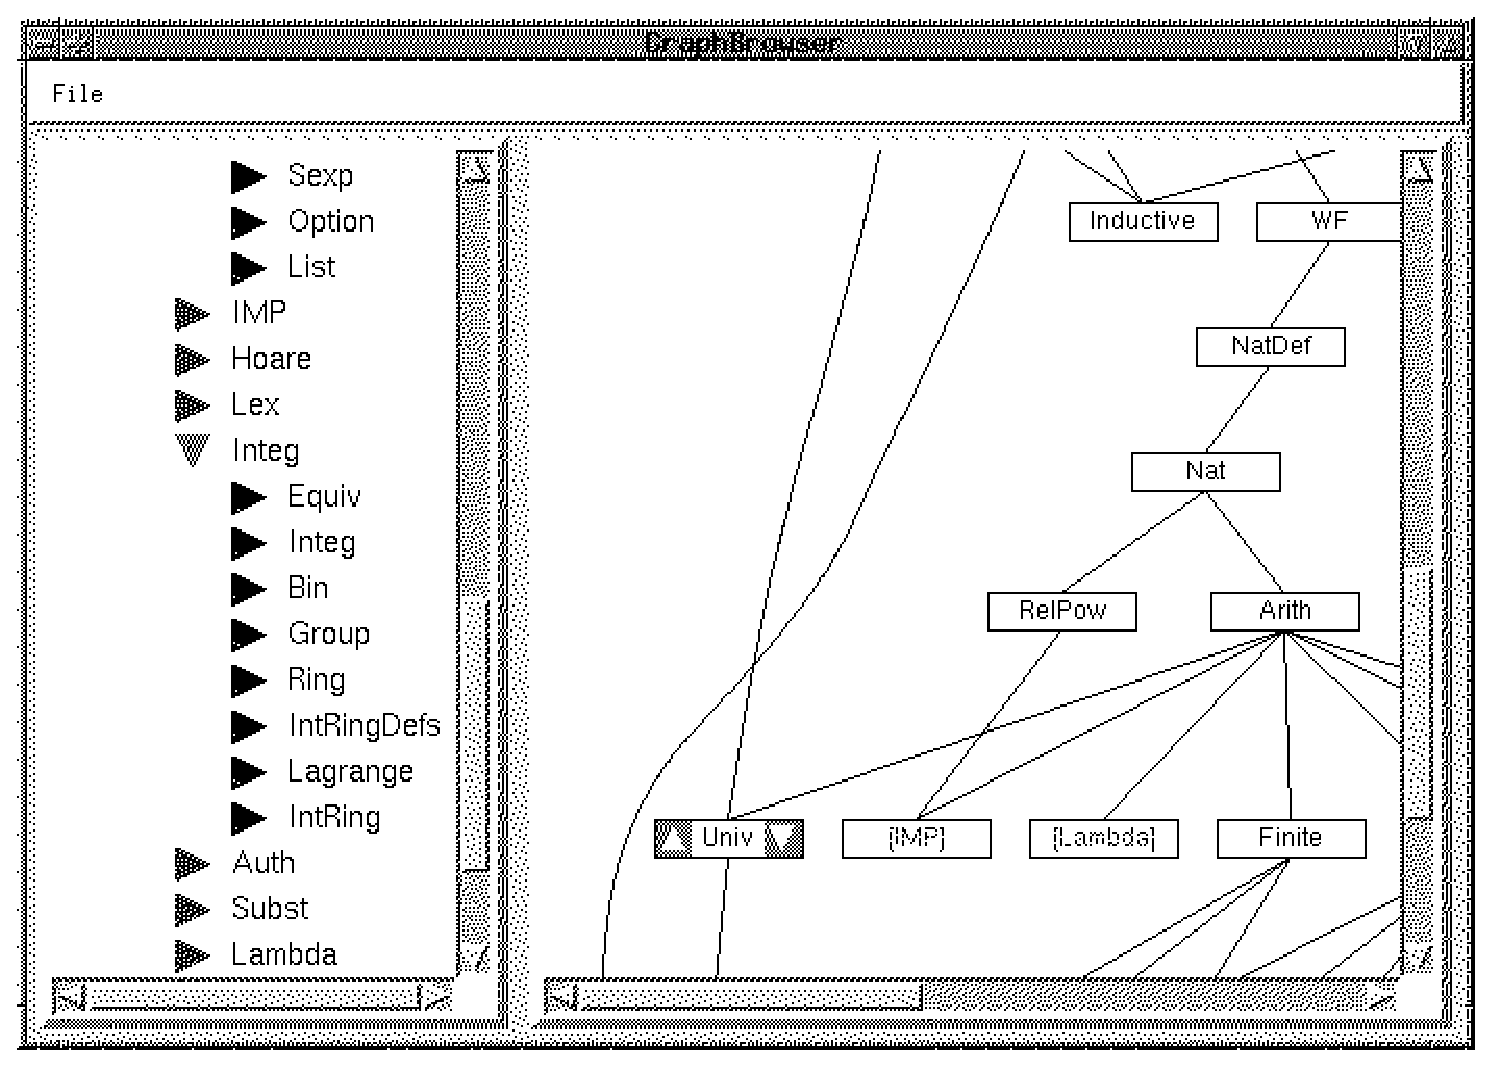
\includegraphics[width=\textwidth]{browser_screenshot}
  \caption{\label{browserwindow} Browser main window}
\end{figure}


\subsubsection*{The directory tree window}

This section describes the usage of the directory browser and the
meaning of the different items in the browser window.
\begin{itemize}
  
\item A red arrow before a directory name indicates that the directory
  is currently ``folded'', i.e.~the nodes in this directory are
  collapsed to one single node. In the right subwindow, the names of
  nodes corresponding to folded directories are enclosed in square
  brackets and displayed in red colour.
  
\item A green downward arrow before a directory name indicates that
  the directory is currently ``unfolded''. It can be folded by
  clicking on the directory name.  Clicking on the name for a second
  time unfolds the directory again.  Alternatively, a directory can
  also be unfolded by clicking on the corresponding node in the right
  subwindow.
  
\item Blue arrows stand before ordinary node (i.e.~theory) names. When
  clicking on such a name, the graph display window focuses to the
  corresponding node. Double clicking invokes a text viewer window in
  which the contents of the theory file are displayed.

\end{itemize}


\subsubsection*{The graph display window}

When pointing on an ordinary node, an upward and a downward arrow is
shown.  Initially, both of these arrows are green. Clicking on the
upward or downward arrow collapses all predecessor or successor nodes,
respectively. The arrow's colour then changes to red, indicating that
the predecessor or successor nodes are currently collapsed. The node
corresponding to the collapsed nodes has the name ``{\tt [....]}''. To
uncollapse the nodes again, simply click on the red arrow or on the
node with the name ``{\tt [....]}''. Similar to the directory browser,
the contents of theory files can be displayed by double clicking on
the corresponding node.


\subsubsection*{The ``File'' menu}

Please note that due to Java security restrictions this menu is not
available in the applet version. The meaning of the menu items is as
follows:
\begin{description}
  
\item[Open$\ldots$] Open a new graph file.
  
\item[Export to PostScript] Outputs the current graph in {\sc
    PostScript} format, appropriately scaled to fit on one single
  sheet of paper.  The resulting file can printed directly.
  
\item[Export to EPS] Outputs the current graph in Encapsulated {\sc
    PostScript} format. The resulting file can be included in other
  documents.

\item[Quit] Quit the graph browser.

\end{description}


\subsection*{*Syntax of graph definition files}

A graph definition file has the following syntax:
\begin{eqnarray*}
  \mbox{\it graph} & = & \{ \: \mbox{\it vertex \tt ;} \: \} ^ + \\
  vertex & = & \mbox{\it vertexname} \: \mbox{\it vertexID} \: \mbox{\it dirname} \: [ \mbox{\tt +} ]
  \: \mbox{\it path} \: [ \mbox{\tt <} | \mbox{\tt >} ] \: \{ \: \mbox{\it vertexID} \: \} ^ *
\end{eqnarray*}

The meaning of the items in a vertex description is as follows:
\begin{description}
  
\item[vertexname] The name of the vertex.
  
\item[vertexID] The vertex identifier. Note that there may be two
  vertices with equal names, whereas identifiers must be unique.
  
\item[dirname] The name of the ``directory'' the vertex should be
  placed in.  A ``{\tt +}'' sign after {\it dirname} indicates that
  the nodes in the directory are initially visible. Directories are
  initially invisible by default.
  
\item[path] The path of the corresponding theory file. This is
  specified relatively to the path of the graph definition file.
  
\item[List of successor/predecessor nodes] A ``{\tt <}'' sign before
  the list means that successor nodes are listed, a ``{\tt >}'' sign
  means that predecessor nodes are listed. If neither ``{\tt <}'' nor
  ``{\tt >}'' is found, the browser assumes that successor nodes are
  listed.

\end{description}


%%% Local Variables: 
%%% mode: latex
%%% TeX-master: "system"
%%% End: 
